\chapter{Problem statement and proposal}\label{B:problemStatementAndProposal}

As this title's chapter sample, the aim of this section is to provide a structured vision of the specific problems of each issue to be developed during this project.

Main issues are about to prepare and/or adapt current technologies to be ready for a cloud deployment. This fact implies studying existing tools in order to create specific microservices that will be interconnected between them. And, finally to carry out required developments in order to assure the goals behind.

--------- splitting the current interface of HTTP requests to TCP socket messages, this means creating the API middleware service that will let configure specific LiveMediaStreamer instances  that loads the audio and video mixer scenario-----------

\section{Architecture study}

Therefore, it's required to define an architecture of the platform to prototype in order to have a global and generic insight. Such architecture should contain the different high level layers as shown next:
\begin{figure}[htb]
\begin{center}
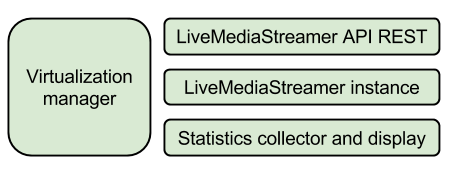
\includegraphics[width=0.35\textwidth]{./images/generalArch.png}
\caption{Generic platform architecture}
\label{F:genericPlatArch}
\end{center}
\end{figure}

The "LiveMediaStreamer API REST" layer will contain the service that will be offered to different and external applications in order to manage the "LiveMediaStreamer instance" layer by creating different audio and video production scenarios. Both layers are the core layers of the platform.

Moreover, in order to offer a centralized monitoring system, the "Statistics collector and display" layer becomes as the box for this requirement.

Finally, it is also required to provide an orchestrator that manages the deployment and distribution of the possible configurations for the previous introduced layers. This will be done thanks to the "Virtualization manager" layer.

\subsection{Virtualization}

This subsection aims to introduce the possibilities that different virtualization technologies could offer for this project requirements and to decide one of them.

First of all, next points are showing which are the expected outcomes for using virtualization and what should fulfill the selected technology:

\begin{itemize}
\item To manage and maintain a system of small pieces of services
\item To have flexibility in order to quickly load required instances (e.g.: to assure real-time scalability)
\item To offer ease to continuous develop and deploy the different parts of the architecture
\item To have version like system for having different version tags for the architecture modules (e.g.: a development and a production box of the same API REST service)
\item To assure full compatibility for the core layers' operating system (right now only Linux environments are supported)
\item To assure full compatibility for the hardware to work with (mainly x86 processors are in the scope)
\end{itemize}

Therefore, it is required to use an as much lightweight as possible technology.

Under Linux environments there are many virtualization options (most of them proprietary) to analyse, but lets focus on the ones that are open-source and have wider and active communities behind.

These are KVM with QEMU and LXC with Docker:

\begin{itemize}
\item KVM (Kernel-based Virtual Machines) \hfill

It's a FreeBSD and Linux kernel module that offers a full virtualization solution for Linux on x86 hardware containing virtualization extensions (Intel VT or AMD-V). It consists of a loadable kernel module that provides the core virtualization infrastructure and a processor specific module.
Usually, KVM runs with the QEMU (Quick Emulator) which is a complete and standalone emulating suite that performs hardware virtualization.

KVM with QEMU is able to offer virtualization for x86, PowerPC, and S/390 guests. For instance, when the target architecture is the same as the host architecture, QEMU can make use of KVM particular features in order to do not emulate CPU nor memory.

--- IMATGE QEMU+KVM---

\item LXC (Linux Containers) \hfill

It's an operating-system-level virtualization environment for running multiple isolated Linux systems (known as containers) on a single Linux central host.

Linux kernel itself provides the cgroups functionality that allows limitation and prioritization of resources (CPU, memory, block I/O, network, etc.) without the need for starting any virtual machines, and namespace isolation functionality that allows complete isolation of an applications' view of the operating environment, including process trees, networking, user IDs and mounted file systems.

Then, the Docker project provides an additional layer of abstraction and automation of operating-system-level virtualization on Linux, Mac OS and Windows.

LXC with Docker is able to 

--- IMATGE DOCKER + LXC ---
\end{itemize}


\subsection{Monitoring layer}
\section{Architecture proposal}
\section{Task planning}



